\chapter{Metodologia}\label{cap:metodologia}

Este capítulo descreve os procedimentos metodológicos empregados no desenvolvimento, otimização e validação experimental do sistema de diagnóstico de falhas em transformadores de potência. Apresenta-se o desenho metodológico estruturado em dois eixos de investigação, fundamentando a divisão operacional a partir das características dos conjuntos de dados industriais disponíveis. Em seguida, detalham-se os procedimentos de auditoria e saneamento das bases de dados, os algoritmos de pré-processamento e engenharia de atributos, a modelagem preditiva temporal por redes neurais recorrentes, a formulação do algoritmo genético aprimorado para otimização do classificador e os protocolos de inferência estatística e interpretabilidade físico-química pós-hoc.

\section{Desenho Metodológico e Arquitetura em Dois Eixos}\label{sec:desenho_metodologico}

A concepção experimental adotada neste estudo decorre de uma restrição objetiva verificada nos repositórios abertos de Análise de Gases Dissolvidos (DGA). Constata-se na literatura uma assimetria insolúvel entre registros temporais contínuos e bases estáticas com anotação abrangente de falhas. As bases temporais disponíveis para acesso público, a exemplo do monitoramento divulgado por \citeonline{katser2022}, fornecem leituras periódicas registradas em intervalos regulares, porém contemplam apenas quatro gases dissolvidos, sem o monitoramento do metano ($\text{CH}_4$) e do etano ($\text{C}_2\text{H}_6$), restringindo os rótulos de integridade operacional a quatro categorias. Em sentido oposto, as bases de classificação que cobrem o conjunto normativo completo de sete estados de operação da IEC 60599 contêm as medições dos cinco gases clássicos, contudo são estruturadas exclusivamente como registros pontuais (instantâneos) coletados no momento da amostragem, inviabilizando o rastreamento longitudinal da taxa de evolução gasosa.

Diante dessa incompatibilidade de variáveis, a pesquisa foi formalmente dividida em dois eixos metodológicos complementares, denominados Track A e Track B, cuja organização geral está esquematizada na Figura~\ref{fig:arquitetura}. O Track A investiga a dimensão temporal da degradação, empregando uma rede neural recorrente do tipo \textit{Long Short-Term Memory} (LSTM) empilhada para modelar a dinâmica multivariada de quatro gases e produzir estimativas futuras de concentração, as quais alimentam um classificador estático XGBoost submetido a estudo formal de ablação da hipótese temporal sobre quatro classes de severidade. O Track B estrutura-se como um referencial comparativo de classificação multiclasse sobre sete categorias de integridade operacional, permitindo confrontar o algoritmo XGBoost otimizado por um Algoritmo Genético Melhorado (IGA) contra os métodos normativos internacionais clássicos, contra referências da literatura recente e contra limites teóricos de informação, integrando ferramentas de explicabilidade agnóstica baseadas em valores de Shapley.

\begin{figure}[htbp]
\centering
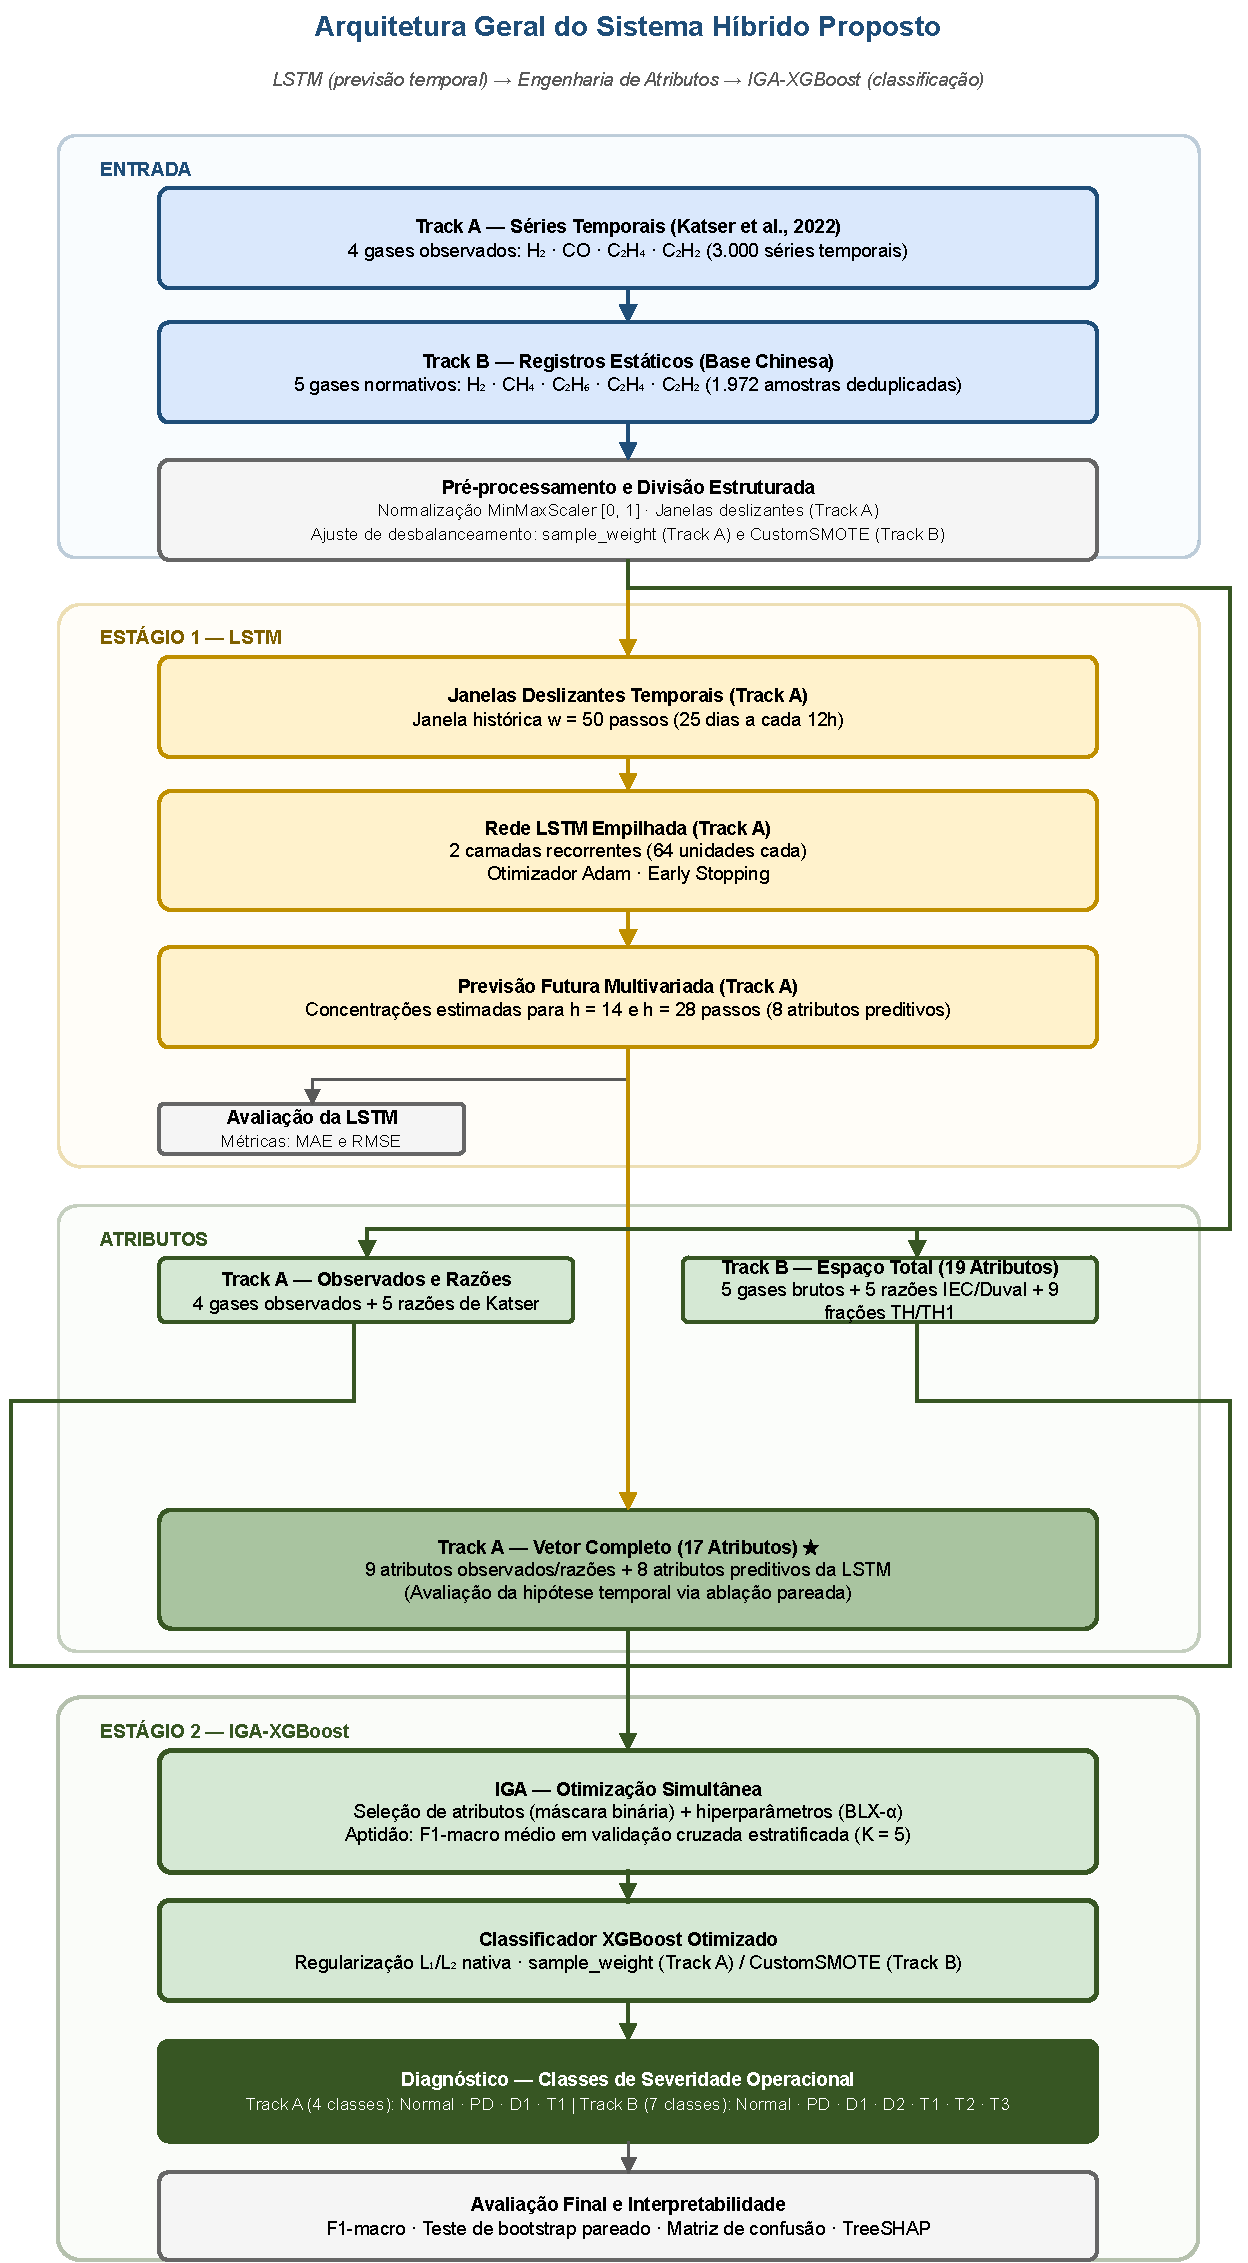
\includegraphics[width=0.85\textwidth]{figuras/Arquitetura.pdf}
\caption{Fluxograma metodológico do trabalho estruturado na bifurcação entre os eixos Track A e Track B.}
\label{fig:arquitetura}
\fonte{Elaborado pelo autor.}
\end{figure}

\section{Bases de Dados e Procedimentos de Auditoria}\label{sec:bases_dados}

A experimentação utiliza dois conjuntos de dados reais e independentes, submetidos a protocolos rigorosos de verificação de integridade e descarte justificado de fontes inconsistentes.

\subsection{Base de Séries Temporais Industriais (Track A)}

O Track A adota o conjunto de dados de telemetria contínua divulgado por \citeonline{katser2022}, proveniente de transformadores de potência em operação contínua em instalações de geração nuclear vinculadas ao consórcio Skoltech e Rosatom. A base é constituída por 3.000 séries temporais multivariadas com amostragem regular a cada 12 horas, totalizando 420 passos temporais por série (210 dias de histórico contínuo). O conjunto oficial encontra-se particionado em 2.100 séries destinadas a treinamento e validação, reservando-se 900 séries exclusivamente para avaliação final de teste independente.

Registram-se nessa base as concentrações de quatro espécies gasosas, compreendendo hidrogênio ($\text{H}_2$), monóxido de carbono ($\text{CO}$), etileno ($\text{C}_2\text{H}_4$) e acetileno ($\text{C}_2\text{H}_2$). Cada série é categorizada por um rótulo terminal que define o estado do equipamento em quatro classes operacionais, distribuídas no teste oficial em 731 instâncias normais (Normal), 38 eventos de descarga parcial (PD), 49 casos de descarga de baixa energia (D1) e 82 ocorrências de sobreaquecimento térmico incipiente (T1). As grandezas reportadas apresentam magnitude reduzida, situando-se na escala de $10^{-3}$, padrão consistente com dados de sensores de monitoramento online contínuo em regime de operação estável, exigindo tratamento analítico para garantia de estabilidade numérica.

\subsection{Base Compilada de Diagnóstico Estático (Track B)}

O Track B utiliza uma compilação de dados estáticos de DGA obtidos a partir de transformadores de potência imersos em óleo mineral em serviço na rede elétrica chinesa. O repositório bruto reúne medições laboratoriais por cromatografia gasosa cobrindo as concentrações absolutas em partes por milhão (ppm) de cinco gases fundamentais, especificamente hidrogênio ($\text{H}_2$), metano ($\text{CH}_4$), etano ($\text{C}_2\text{H}_6$), etileno ($\text{C}_2\text{H}_4$) e acetileno ($\text{C}_2\text{H}_2$), acompanhados pelo laudo confirmado de integridade estrutural.

Durante a etapa de auditoria dos dados brutos, constatou-se que o repositório original de 2.321 amostras apresentava 349 registros rigorosamente duplicados em todos os atributos e rótulos, representando uma taxa de redundância de 15,0\%. A permanência dessas duplicatas violaria o princípio de independência amostral, gerando contaminação mútua entre dobras de validação cruzada e sobrestimando a acurácia dos modelos. Conduziu-se um processo compulsório de deduplicação, resultando em 1.972 instâncias únicas e não viesadas. Essa base consolidada foi dividida de maneira estratificada em conjunto de treinamento com 1.477 amostras (74,9\%), conjunto de validação com 200 amostras (10,1\%) e partição de teste independente com 295 amostras (15,0\%). As amostras distribuem-se entre as sete classes normativas da IEC 60599, sendo 707 normais, 111 de descargas parciais (PD), 273 de descargas de baixa energia (D1), 221 de descargas de alta energia (D2), 107 de sobreaquecimentos inferiores a 300~$^\circ\text{C}$ (T1), 108 de falhas térmicas entre 300~$^\circ\text{C}$ e 700~$^\circ\text{C}$ (T2) e 435 de falhas térmicas severas superiores a 700~$^\circ\text{C}$ (T3).

\subsection{Critérios de Exclusão e Descarte de Bases de Dados}

O refinamento metodológico exigiu o descarte justificado de fontes de dados consideradas em etapas preliminares da pesquisa. Descartou-se a base descrita em estudos de previsão temporal por \citeonline{wang2023} após constatação de sua indisponibilidade pública, tratando-se de acervo proprietário de concessionária sob termo de sigilo industrial. Do mesmo modo, registros citados com volume estrito de 430 amostras associados a trabalhos correlatos foram reavaliados em virtude de divergências na literatura quanto à proveniência física e critérios de anonimização.

Adicionalmente, rejeitou-se o uso de métodos de simulação estatística por Monte Carlo para geração de amostras sintéticas completas de DGA. A dispersão estocástica gerada artificialmente tende a mascarar a correlação físico-química intrínseca que governa a quebra molecular do óleo isolante, criando distribuições homogêneas inexistentes na realidade de campo. A opção por bases exclusivamente empíricas auditadas preserva a integridade das relações estequiométricas e fundamenta a credibilidade científica das inferências.

\section{Pré-processamento e Engenharia de Atributos}\label{sec:preprocessamento}

Os registros de gases dissolvidos demandam transformações matemáticas destinadas a compatibilizar amplitudes e evidenciar padrões cinéticos de degradação.

\subsection{Tratamento de Escala e Normalização}

As concentrações gasosas em transformadores de potência exibem assimetria estatística acentuada, com a maioria dos equipamentos operando com concentrações residuais próximas a zero, enquanto falhas de arco elétrico ou sobreaquecimentos graves induzem picos de hidrogênio e etileno superiores a dezenas de milhares de ppm. Para atenuar a amplitude dessas caudas pesadas sem truncamento de informação, aplicou-se aos dados observados a transformação logarítmica com deslocamento unitário, expressa por $x_{\text{log}} = \ln(x + 1)$, na qual o incremento unitário assegura a convergência da função para registros com concentração nula.

Subsequentemente, as grandezas transformadas foram mapeadas para o intervalo contínuo $[0, 1]$ por meio de reescalonamento linear Min-Max, definido por $(x_{\text{log}} - x_{\text{min}}) / (x_{\text{max}} - x_{\text{min}})$. Para assegurar rigor metodológico e evitar qualquer forma de vazamento de informação entre partições, os extremos de escala $x_{\text{min}}$ e $x_{\text{max}}$ foram ajustados estritamente sobre as partições de treinamento, aplicando-se os escaladores previamente ajustados às amostras de validação e teste.

\subsection{Espaço de Atributos do Track A}

Para o Track A, estruturou-se um espaço vetorial candidato contendo 17 variáveis explicativas, distribuídas em três categorias funcionais. A primeira categoria compreende os quatro gases brutos observados instantaneamente ($\text{H}_{2,\text{obs}}$, $\text{CO}_{\text{obs}}$, $\text{C}_2\text{H}_{4,\text{obs}}$ e $\text{C}_2\text{H}_{2,\text{obs}}$). A segunda categoria reúne razões químicas adaptadas à disponibilidade da base, incluindo a razão clássica $\text{C}_2\text{H}_2/\text{C}_2\text{H}_4$, a razão adaptada $\text{H}_2/\text{C}_2\text{H}_2$, a soma total de hidrocarbonetos adaptada aos gases monitorados ($\text{TH}_{\text{katser}} = \text{C}_2\text{H}_4 + \text{C}_2\text{H}_2$) e as respectivas proporções parciais $\text{C}_2\text{H}_2/\text{TH}_{\text{katser}}$ e $\text{C}_2\text{H}_4/\text{TH}_{\text{katser}}$. Cabe assinalar que a razão $\text{CO}/\text{C}_2\text{H}_4$, inicialmente cogitada em estudos preliminares, foi expurgada da modelagem após auditoria físico-química, uma vez que monóxido de carbono e etileno derivam de mecanismos de pirólise termicamente independentes, correspondendo respectivamente à isolação sólida celulósica e ao óleo mineral, sem relação de proporcionalidade estequiométrica em normas reconhecidas.

A terceira categoria engloba oito atributos prospectivos gerados pelo módulo recorrente LSTM, correspondendo às projeções de concentração de cada um dos quatro gases para os horizontes operacionais de uma semana ($h = 14$ passos) e duas semanas ($h = 28$ passos), designados por $\text{H}_{2,\text{h14}}$, $\text{CO}_{\text{h14}}$, $\text{C}_2\text{H}_{4,\text{h14}}$, $\text{C}_2\text{H}_{2,\text{h14}}$, $\text{H}_{2,\text{h28}}$, $\text{CO}_{\text{h28}}$, $\text{C}_2\text{H}_{4,\text{h28}}$ e $\text{C}_2\text{H}_{2,\text{h28}}$.

\subsection{Espaço de Atributos do Track B}

Para a classificação de sete classes do Track B, construiu-se um espaço amostral de 19 atributos candidatos fundamentados nas diretrizes da IEC 60599, no método de Doernenburg e na formulação empírica estendida de \citeonline{wu2021}. O vetor incorpora as cinco concentrações originais ($\text{H}_2$, $\text{CH}_4$, $\text{C}_2\text{H}_6$, $\text{C}_2\text{H}_4$ e $\text{C}_2\text{H}_2$), as quatro razões de diagnóstico normatizadas ($\text{CH}_4/\text{H}_2$, $\text{C}_2\text{H}_2/\text{C}_2\text{H}_4$, $\text{C}_2\text{H}_4/\text{C}_2\text{H}_6$ e $\text{C}_2\text{H}_2/\text{CH}_4$), e a família de coordenadas do Triângulo 1 de Duval baseada na soma dos três gases que definem o espaço triangular ($\text{TH} = \text{CH}_4 + \text{C}_2\text{H}_4 + \text{C}_2\text{H}_2$), gerando as proporções $\% \text{CH}_4/\text{TH}$, $\% \text{C}_2\text{H}_4/\text{TH}$ e $\% \text{C}_2\text{H}_2/\text{TH}$.

Adicionou-se ainda a família de atributos proposta por \citeonline{wu2021}, calculada sobre a soma total de hidrocarbonetos ($\text{TH}_1 = \text{CH}_4 + \text{C}_2\text{H}_6 + \text{C}_2\text{H}_4 + \text{C}_2\text{H}_2$), contemplando a razão $\text{C}_2\text{H}_2/\text{C}_2\text{H}_6$ e os quatro percentuais relativos calculados sobre $\text{TH}_1$. A todos os denominadores de razões incorporou-se um valor infinitesimal $\epsilon = 10^{-5}$ para evitar singularidades numéricas de divisão por zero.

\subsection{Tratamento do Desbalanceamento de Classes}

O desbalanceamento numérico entre falhas raras e o regime de operação normal exige compensação algorítmica para evitar que a função de perda favoreça a classe majoritária. No presente trabalho, adotou-se a estratégia de ponderação analítica no treinamento multiclasse mediante o parâmetro de custo diferencial por instância (\texttt{sample\_weight}) no algoritmo XGBoost. O peso associado a cada amostra pertencente à classe $c$ foi definido pelo inverso de sua frequência relativa na partição de treino, expresso por $w_c = N / (C \cdot N_c)$, no qual $N$ denota o número total de amostras de treinamento, $C$ representa o total de categorias e $N_c$ indica o contingente da classe em questão.

Essa abordagem preserva as instâncias reais observadas sem distorcer as relações geométricas entre gases brutos e razões derivadas. A aplicação de técnicas de superamostragem sintética baseadas em interpolação linear clássica foi preterida em virtude de sua inadequação teórica para dados que combinam grandezas aditivas e não lineares, haja vista que médias lineares de razões não coincidem com as razões das médias lineares de concentração.

\section{Módulo de Previsão Temporal}\label{sec:modulo_lstm}

O primeiro estágio de processamento no Track A consiste em uma rede neural recorrente LSTM empilhada, projetada para aprender a evolução temporal dos gases e extrapolar suas trajetórias para horizontes futuros. As séries temporais são estruturadas por meio da técnica de janela deslizante multivariada. Considerando o vetor observacional no passo discreto $t$, a matriz de entrada do modelo é formada pelo histórico de $w = 50$ passos regulares contíguos (equivalente a 25 dias de operação), configurando uma matriz de dimensão $50 \times 4$. O alvo do aprendizado supervisionado consiste no vetor com as quatro concentrações no passo $t + h$, onde $h$ denota o horizonte preditivo recursivo.

A topologia da rede compreende duas camadas recorrentes LSTM empilhadas em cascata com 64 unidades ocultas cada, dotadas de funções de ativação por tangente hiperbólica e portas recorrentes com função sigmoide. Para reduzir o risco de sobreajuste durante o treinamento, intercalou-se entre as camadas uma regularização por \textit{dropout} com probabilidade de 0,2. A camada final consiste em uma estrutura densa linear com quatro unidades correspondentes às estimativas pontuais dos quatro gases.

O treinamento foi configurado com o otimizador Adam sob taxa de aprendizado inicial de $10^{-3}$, minimizando o erro quadrático médio (MSE) com lotes de 1.024 amostras. O ajuste hiperparamétrico incorporou mecanismo de redução dinâmica da taxa de aprendizado em patamares (\texttt{ReduceLROnPlateau}), aplicando decaimento de 0,5 após sete épocas sucessivas sem decréscimo da perda de validação, associado a critério de parada antecipada com paciência fixada em 15 épocas. Para avaliar a extensão temporal da capacidade de previsão do modelo, foram calculados recursivamente 11 horizontes preditivos distintos, abrangendo $h \in \{1, 2, 4, 7, 14, 28, 42, 56, 70, 84, 98\}$ passos (de 12 horas a 7 semanas de extrapolação contínua), selecionando-se os horizontes de $h = 14$ e $h = 28$ passos para alimentação do classificador.

\section{Algoritmo Genético Melhorado e Otimização do XGBoost}\label{sec:iga_xgboost}

Para automatizar a busca por arquiteturas parcimoniosas no segundo estágio da arquitetura, implementou-se uma versão personalizada do Algoritmo Genético Melhorado (IGA) com suporte da biblioteca DEAP (\textit{Distributed Evolutionary Algorithms in Python}). O algoritmo executa a seleção de subconjuntos informativos de variáveis e sintoniza simultaneamente os hiperparâmetros contínuos do modelo XGBoost.

\subsection{Representação Cromossômica e Operadores Genéticos}

Cada indivíduo da população evolutiva é codificado por uma estrutura cromossômica heterogênea bipartida. A primeira porção é definida por uma máscara binária de dimensão $p$, na qual o bit unitário indica a inclusão da respectiva variável diagnóstica e o bit nulo indica sua exclusão da matriz de treinamento do XGBoost. A segunda porção é composta por nove genes contínuos reais normalizados no intervalo $[0, 1]$, mapeados linearmente para as escalas de busca dos hiperparâmetros estruturais do ensemble de árvores. Os intervalos definidos cobrem a taxa de aprendizado (\texttt{learning\_rate} entre 0,01 e 0,30), a profundidade máxima das árvores (\texttt{max\_depth} de 3 a 10), o número de estimadores (\texttt{n\_estimators} de 50 a 500), as frações de amostragem (\texttt{subsample} e \texttt{colsample\_bytree} entre 0,50 e 1,00), o ganho mínimo para divisão de nós (\texttt{gamma} de 0,0 a 1,0), o peso mínimo foliar (\texttt{min\_child\_weight} de 1 a 10) e os termos de regularização $L_1$ e $L_2$ (\texttt{reg\_alpha} e \texttt{reg\_lambda} entre 0,0 e 10,0).

O processo reprodutivo adota operadores probabilísticos combinados. Para a porção binária de seleção de atributos, aplica-se cruzamento uniforme com recombinação independente de variáveis. Para a porção contínua de hiperparâmetros, emprega-se o operador de cruzamento binário simulado (\textit{Simulated Binary Crossover}, SBX) com índice de distribuição $\eta_c = 20$. As mutações atuam por inversão pontual de bits na máscara binária e por perturbação polinomial gaussiana nos genes contínuos. A seleção dos progenitores opera por torneio com tamanho $k = 3$, preservando-se estritamente os dois melhores indivíduos de cada geração por elitismo direto.

\subsection{Função de Aptidão e Critérios de Parada}

A avaliação de aptidão (\textit{fitness}) orienta-se pela maximização do desempenho preditivo balanceado. Considerando o desbalanceamento das categorias operacionais, adota-se como métrica orientadora o $F_1$-macro médio obtido por validação cruzada estratificada em 5 dobras ($K = 5$) computada estritamente sobre as amostras de treinamento. Adicionalmente, aplica-se uma penalização marginal de parcimônia dimensional para privilegiar representações compactas que descartem variáveis colineares, conforme estabelecido na Equação~(\ref{eq:fitness_metodologia}).

\begin{equation}\label{eq:fitness_metodologia}
f(\mathbf{c}) = F1_{\text{macro}}^{CV} - \lambda \cdot \frac{k}{p}
\end{equation}

Em que $\mathbf{c}$ representa o cromossomo sob avaliação, $F1_{\text{macro}}^{CV}$ indica o macro-escore harmônico médio nas dobras internas de validação, $k$ corresponde à quantidade de atributos ativos na máscara, $p$ representa a quantidade total de atributos candidatos disponíveis e $\lambda = 0,005$ configura o coeficiente de parcimônia. A evolução foi configurada com população de 50 indivíduos por até 100 gerações, incorporando critério de parada antecipada com tolerância fixada em 20 gerações consecutivas sem melhoria na melhor aptidão global.

\section{Protocolo Experimental e Rigor Estatístico}\label{sec:protocolo_experimental}

Para blindar as conclusões contra aleatoriedade amostral e evitar conclusões espúrias, desenhou-se um protocolo experimental estruturado em testes de ablação pareados e avaliações repetidas de teto informacional.

\subsection{Desenho Experimental e Ablação no Track A}

O desenho experimental do Track A foi estruturado para isolar matematicamente o efeito individual exercido pelas previsões temporais da rede LSTM sobre a capacidade discriminativa estática. Para tanto, definiram-se cinco configurações experimentais controladas. A configuração C2 estabelece o classificador XGBoost padrão operando sobre o conjunto completo de 17 atributos (quatro gases observados, cinco razões adaptadas e oito previsões da LSTM para $h=14$ e $h=28$). A configuração C1 aplica o IGA sobre o mesmo espaço de 17 atributos candidatos, selecionando recursivamente atributos e hiperparâmetros. A configuração C5a adota os hiperparâmetros padrão do XGBoost restritos aos 9 atributos estáticos observados, sem qualquer fornecimento de variáveis da LSTM. A configuração C5b avalia o IGA restrito aos 9 atributos estáticos observados, executando otimização evolutiva autônoma sem acesso à dimensão temporal. Por fim, a configuração C6 avalia o XGBoost padrão treinado unicamente com as 8 variáveis preditivas geradas pela LSTM.

\subsection{Desenho Experimental no Track B}

No Track B, o protocolo investiga o comportamento dos modelos frente ao diagnóstico multiclasse de sete estados operacionais. A configuração C3 corresponde ao modelo proposto IGA-XGBoost avaliado sobre os 19 atributos candidatos. A configuração C4 utiliza o XGBoost com parametrização padrão sobre os mesmos 19 atributos. A configuração T3 replica fielmente o modelo de referência de \citeonline{wu2021}, combinando 18 variáveis estendidas e busca por IGA. As configurações T2 e T1 avaliam as regras normativas tradicionais do Triângulo 1 de Duval e do Método das Razões da IEC 60599, respectivamente, implementadas em conformidade analítica com as tabelas das normas vigentes.

\subsection{Procedimentos de Bootstrap Pareado e Validação Cruzada Repetida}

A quantificação de significância estatística prescindiu de premissas paramétricas de normalidade assintótica. Para a avaliação no conjunto de teste, aplicou-se o método de reamostragem por \textit{bootstrap} pareado com 5.000 iterações independentes com reposição sobre as amostras de teste. Em cada iteração $b$, computaram-se o índice $F_1$-macro de cada modelo e a diferença pareada exata $\Delta F_1 = F_1(A) - F_1(B)$, construindo-se a distribuição empírica das diferenças. Os intervalos de confiança empíricos com nível de 95\% foram determinados pelos percentis 2,5\% e 97,5\% dessa distribuição. A hipótese nula de equivalência diagnóstica é rejeitada somente quando o intervalo de confiança exclui a linha de nulidade ($\Delta F_1 = 0$) e o valor $p$ aproximado pelo teste bicaudal satisfaz $p < 0,05$.

Complementarmente, com o intuito de investigar a estabilidade e a existência de teto informacional na base do Track B, os modelos C3, C4, T3 e a linha de base sobre os gases primários brutos foram submetidos a validação cruzada estratificada repetida em cinco repetições com cinco dobras (\textit{Repeated Stratified K-Fold} $5 \times 5$, totalizando 25 dobras de treino e teste), computando-se médias e desvios consolidados para verificar a sobreposição dos intervalos de confiança paramétricos.

\section{Protocolo de Interpretabilidade e Validação Físico-Química}\label{sec:protocolo_interpretabilidade}

Para validar a conformidade dos padrões aprendidos pelos ensembles de árvores com os princípios fundamentais da degradação termodinâmica de óleos isolantes, estabeleceu-se um arcabouço de inteligência artificial explicável baseado na formulação de TreeSHAP aditivo \cite{lundberg2020}. Os valores de Shapley foram computados diretamente pelo algoritmo nativo do XGBoost (\texttt{pred\_contribs}), que decomprime as contribuições marginais de cada variável sobre o espaço aditivo contínuo de log-odds de cada classe, satisfazendo localmente a propriedade axiomática de eficiência pela qual a soma das importâncias individuais acrescida do viés basal de classe reproduz a margem contínua de decisão da árvore.

O protocolo de interpretabilidade contempla cinco procedimentos encadeados. O primeiro avalia a estabilidade estocástica do ordenamento de importância mediante o coeficiente de correlação de postos de Spearman ($\rho$) calculado entre os vetores médios de importância absoluta extraídos a partir de modelos ajustados sob cinco sementes aleatórias distintas, considerando valores de $\rho > 0,80$ indicativos de relevância robusta. O segundo procedimento agrupa a contribuição dos atributos em quatro famílias químicas funcionais (derivados de acetileno, etileno, metano e gases brutos), permitindo analisar a alocação de crédito sem distorção induzida por colinearidade entre variáveis aparentadas.

O terceiro procedimento emprega a matriz de interações de Lundberg (\texttt{pred\_interactions}) para isolar o efeito principal univariado ($\phi_{i,i}$), descartando os termos de interação mútua de segunda ordem. Essas curvas de contribuição marginal foram desnormalizadas para a escala física original das concentrações e razões, permitindo identificar os pontos de transição em que o impacto marginal passa de inibidor para promotor de determinada falha ($\phi_{i,i} = 0$) e confrontá-los com as linhas de corte analíticas das normas de Duval e IEC 60599. O quarto procedimento projeta espacialmente os erros de classificação sobre as coordenadas triangulares do Triângulo 1 de Duval, permitindo verificar a concentração espacial dos equívocos diagnósticos nas fronteiras poligonais. Por fim, o quinto procedimento examina a migração estocástica de crédito de importância através de análises de decomposição em instâncias onde variáveis observadas e projetadas pela LSTM competem pela partição do ganho informacional das árvores.
